\definecolor{eps-node-color-1}{HTML}{B0B0B0}
\begin{figure}[t]
\centering
\definecolor{top-node-color}{HTML}{3e5561}
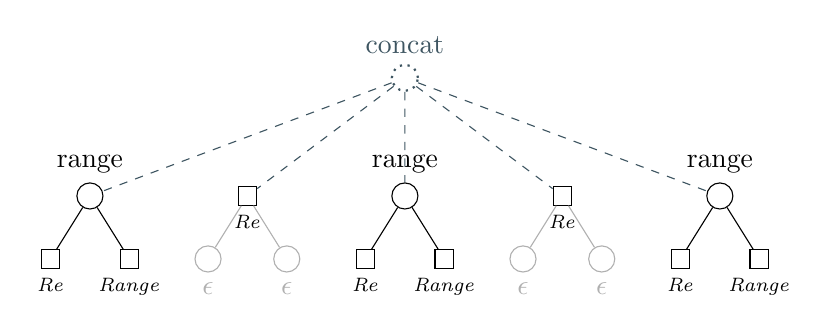
\begin{tikzpicture}[
level 1/.style={sibling distance=2cm},
level 2/.style={sibling distance=1cm},
level 1/.append style={level distance=1.5cm},
level 2/.append style={level distance=.8cm},
empty/.style={edge from parent/.style={solid,eps-node-color-1,draw}}]
\tikzstyle{every node}=[circle,draw=black, solid, edge from parent/.style={solid,eps-node-color-1,draw=black}]
\tikzstyle{edge from parent}=[draw=black, solid]
\tikzstyle{every label}=[rectangle, draw=none]

\node (Root) [label={[text=top-node-color]:concat}, draw=top-node-color,thick, dotted] {} 
child {
    node [label={range}] {} edge from parent[draw=top-node-color,dashed]
    child {
        node [label=below:{\scriptsize\textit{Re}}, draw=black, rectangle] {} }
    child {
        node [label=below:{\scriptsize\textit{Range}}, draw=black, rectangle] {} }
}
%
child {
    node [label=below:{\scriptsize\textit{Re}}, rectangle] {} edge from parent[draw=top-node-color,dashed]
    child[empty] {
        node [label={[text=eps-node-color-1]below:\(\epsilon\)}, draw=eps-node-color-1] {}}
    child[empty] {
        node [label={[text=eps-node-color-1]below:\(\epsilon\)}, draw=eps-node-color-1] {}}
}
%
child {
    node [label={range}] {} edge from parent[draw=top-node-color,dashed]
    child {
        node [label=below:{\scriptsize\textit{Re}}, draw=black, rectangle] {} }
    child {
        node [label=below:{\scriptsize\textit{Range}}, draw=black, rectangle] {} }
}
%
child {
    node [label=below:{\scriptsize\textit{Re}}, rectangle] {} edge from parent[draw=top-node-color,dashed]
    child {
        node [label={[text=eps-node-color-1]below:\(\epsilon\)}, draw=eps-node-color-1] {}  edge from parent[draw=eps-node-color-1] }
    child {
        node [label={[text=eps-node-color-1]below:\(\epsilon\)}, draw=eps-node-color-1] {}  edge from parent[draw=eps-node-color-1] }
}
%
child {
    node [label={range}] {}edge from parent[draw=top-node-color,dashed]
    child {
        node [label=below:{\scriptsize\textit{Re}}, draw=black, rectangle] {} }
    child {
        node [label=below:{\scriptsize\textit{Range}}, draw=black, rectangle] {} }
};

\end{tikzpicture}
\caption{Sketch multi-tree whose completion results in \UseVerb{date2}.}
\label{fig:date-sketch-multitree}
\end{figure}{}